\subsection{Development Methodology and SDLC Approach}

An incremental SDLC approach with agile characteristics was adopted. The project did not follow a strict waterfall model because intent labels, routing rules, UI requirements, and monitoring needs changed during implementation. However, the work remained structured through a repeating cycle of requirement clarification, implementation, test execution, issue logging, correction, and documentation.

This approach was reflected in the issue log maintained during development. Problems such as incorrect route priority, stale asset loading, model-selection edge cases, and missing admin diagnostics were recorded and then addressed in subsequent iterations. From an SDLC perspective, the project therefore moved through the classic stages of requirements analysis, design, implementation, testing, deployment, and maintenance, but with feedback loops between them rather than one strictly linear pass.

\subsection{Requirements and Functional Decomposition}

The project requirements were divided into five main capability groups.

First, a machine learning layer was required to classify user utterances into haematology-relevant intents. Second, a response layer was required to deliver safe and relevant answers without relying on unrestricted generation. Third, a web application layer was required to expose the assistant through an accessible chat interface. Fourth, an operational layer was required to record production traffic, flagged phrases, and review decisions. Fifth, a retraining layer was required to convert reviewed user phrases into future training data.

These requirements were then decomposed into concrete modules: data utilities, training pipeline, inference registry, entity detection, retrieval engine, routing engine, API endpoints, browser UI, PostgreSQL store, admin console, review export tools, and retraining scripts.

\begin{figure}[H]
    \centering
    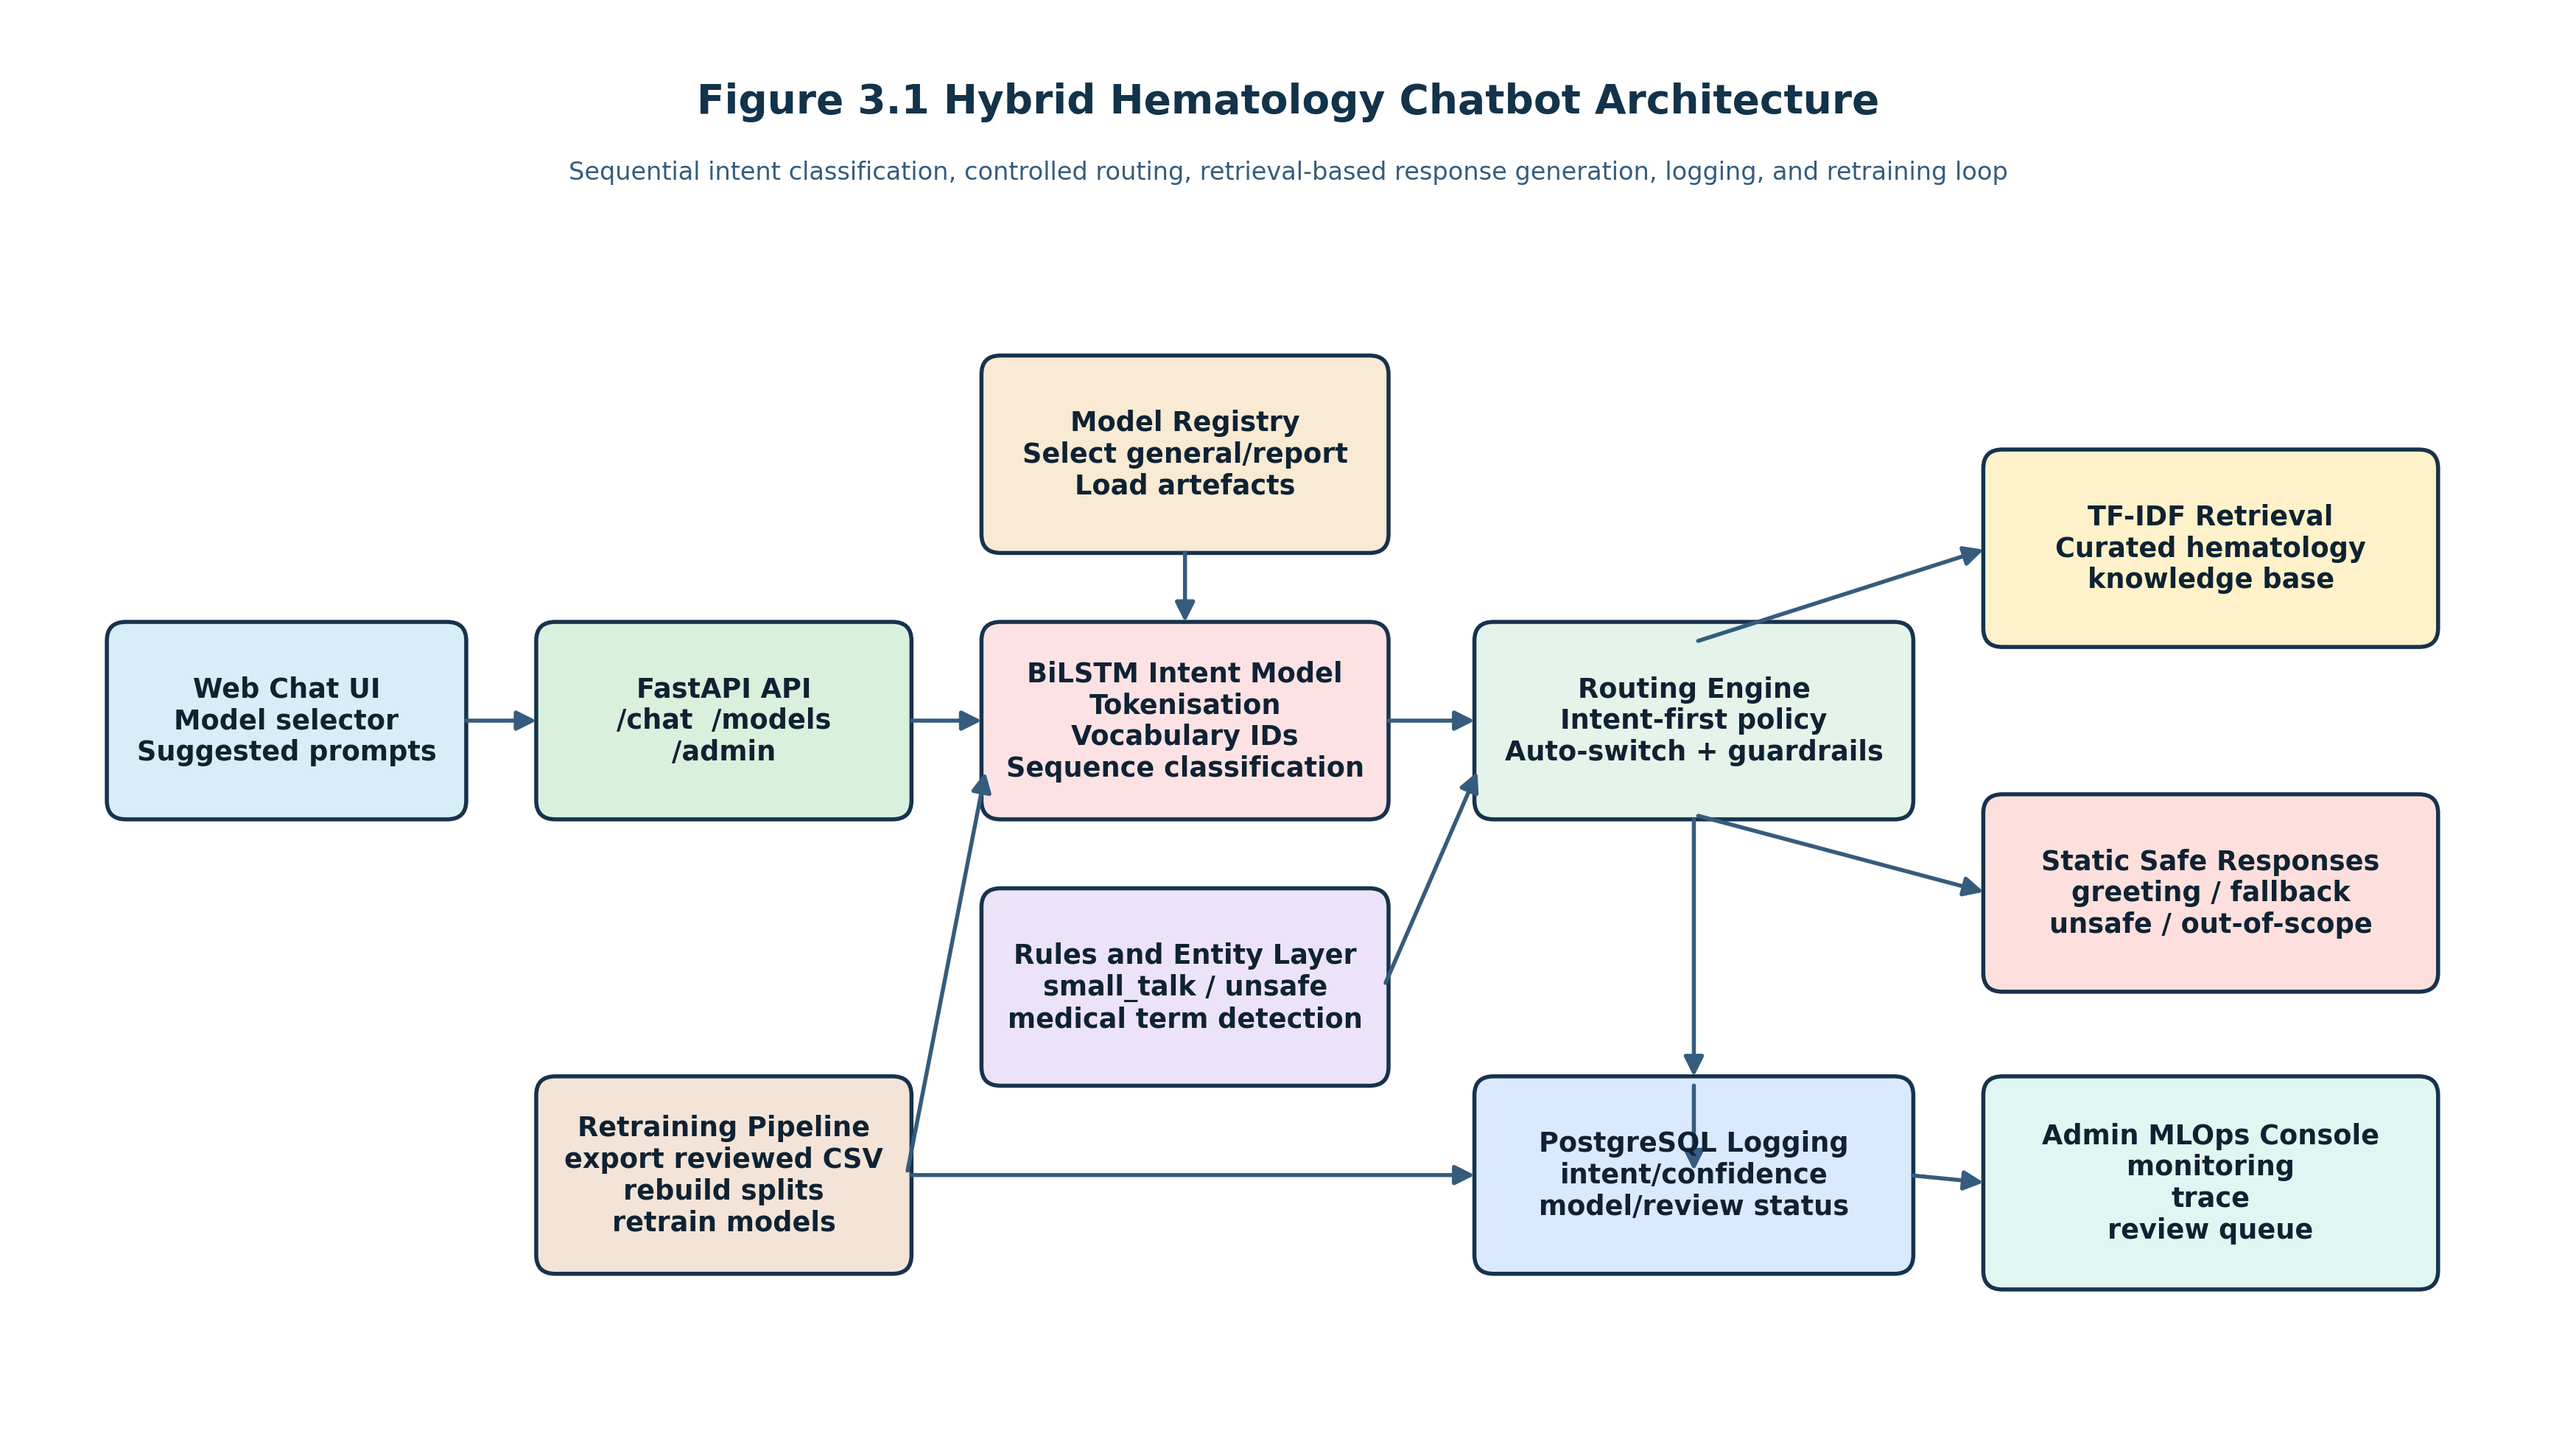
\includegraphics[width=0.9\linewidth]{figures/hybrid_architecture.png}
    \caption{Hybrid haematology chatbot architecture.}
    \label{fig:hybrid-architecture}
\end{figure}

The system was implemented as a hybrid pipeline. A user message was first submitted from the browser UI to a FastAPI backend. A model selector determined whether the \texttt{general} or \texttt{report} profile should be used, with automatic switching when the requested model did not match the detected scope. The selected BiLSTM predictor then normalised the text, tokenised it, converted tokens into vocabulary indices, padded the sequence, and produced intent probabilities. After intent prediction, routing logic decided whether the answer should come from a static control response or the retrieval layer. Entity detection could refine retrieval within broad medical intents, but was constrained from overriding already-specific operational intents.

\subsection{Dataset Design and Growth Strategy}

The dataset strategy was central to the project. Rather than relying on a single fixed file, the data lifecycle was divided into reusable stages. Raw inputs were kept separate from labelled phrase files. A master training dataset was then built from labelled inputs, and model-specific datasets were derived from that master file. Fixed train, validation, and test splits were then generated from the derived datasets.

At the time of final documentation, the master dataset contained 5,391 labelled utterances across 29 intents. The general model dataset contained 2,670 utterances across 21 intents, while the report model dataset contained 4,777 utterances across 26 intents. Large classes included \texttt{cbc\_info=312}, \texttt{coag\_test=300}, \texttt{sample\_collection=214}, and \texttt{report\_numeric\_result\_analysis=1,219}. Additional data was added iteratively to improve weak classes such as \texttt{small\_talk}, \texttt{capability\_query}, \texttt{coag\_test}, and multi-value report-analysis prompts.

The design rationale for two model profiles was straightforward. The \texttt{general} model was intended for workflow, specimen handling, QC, coagulation, smear, and communication intents. The \texttt{report} model was intended for CBC parameter, flag, abnormality, and report-structure support. Some vocabulary overlap was expected because both models operated in the same domain. However, separate datasets reduced label competition between workflow questions and report-reading questions.

\subsection{Preprocessing Pipeline}

Text preprocessing was kept explicit and inspectable. Input text was normalised and tokenised into simple lexical units. A vocabulary was built from the training split, and each token was converted into an integer index. Sequences were then padded to a fixed maximum length so that they could be batched efficiently. A train-validation-test split of 70/15/15 was adopted and fixed on disk for reproducibility. The general split produced 1,868 training rows, 401 validation rows, and 401 test rows. The report split produced 3,343 training rows, 717 validation rows, and 717 test rows after the report-analysis expansions.

This split-aware process was introduced because earlier single-holdout evaluation made it difficult to distinguish model selection from final testing. By separating validation from test, the best checkpoint could be chosen using validation F1 while leaving the test set untouched for final reporting.

\subsection{Sequential Model Design}

The intent classifier was implemented as a BiLSTM with an embedding layer, recurrent sequence encoder, and classification head. The input sequence was embedded into dense vectors, processed bidirectionally, pooled, and then projected to the intent label space. In NLP terms, this stage performed token-sequence modelling over a bounded vocabulary rather than free-text generation. Training used batch size 64, learning rate 0.001, weight decay 1e-05, and 8 epochs in the reported runs.

The general model reached its best validation F1 at epoch 7 with a validation F1 of 0.8978. After the report-analysis and multi-value expansions, the report model also reached its best validation F1 at epoch 7, where validation F1 rose to 0.9444 on the larger report dataset. These results suggested that the models were learning useful structure without severe early overfitting. However, the gap between validation and test performance indicated that the datasets were still moderately challenging and somewhat imbalanced.

\subsection{Retrieval Layer and Knowledge Base}

The knowledge base was stored as curated haematology response entries in JSONL format. Each entry linked an intent and a canonical question to an approved answer. A TF-IDF retrieval layer with unigram and bigram weighting ranked candidate answers against the user utterance and returned the highest-scoring match within the permitted intent scope. Cosine similarity was then used to score the overlap between the user phrase and the curated knowledge entries.

This design had several advantages. First, response text remained controlled and auditable. Second, exact knowledge gaps could be addressed by adding or editing individual entries without retraining the neural model. Third, the retrieval layer could be traced visibly in the admin panel by showing candidate matches and similarity scores. Fourth, the retrieval engine operated within the predicted intent, which reduced the risk of broad but semantically plausible answers crossing into the wrong operational scope.

The main trade-off was that answer quality depended heavily on knowledge-base coverage. If a specific question had not been represented in the curated answer store, the classifier could still be correct while the final answer remained too general. This happened during development with specimen rejection, CBC tube questions, and report-analysis prompts, and was corrected by expanding retrieval entries, introducing a bounded report-analysis layer, and tightening route priority.

\subsection{Safety Rules, Communication Intents, Model Switching, and Report Analysis}

The project implemented dedicated intents for greeting, thanks, goodbye, small talk, clarification, capability questions, incomplete queries, out-of-scope prompts, and unsafe medical requests. This design avoided a common chatbot failure in which non-medical phrases are forced artificially into medical classes. In NLP terms, these intents were handled through a mixture of learned classification and rule-priority short-circuiting so that high-risk phrases did not depend only on the softmax output of the BiLSTM.

A separate model advisory and auto-switch mechanism was also introduced. If a user selected the \texttt{general} model but asked a report-oriented question, the request could be answered by the \texttt{report} model instead. Conversely, if the \texttt{report} model was selected for a workflow question such as specimen tube handling, the system could switch back to the \texttt{general} model. This improved usability without requiring the user to understand the internal architecture.

An additional NLP layer was added for report analysis. Report-like phrases such as \texttt{WBC is 13.7}, \texttt{My report shows anemia}, or \texttt{Age is 50 WBC is 13 MCV is 73 PLT is 1} could not be handled reliably through pure intent classification alone because they required lightweight information extraction after the intent had been recognised. A bounded report-analysis module was therefore implemented to extract analyte labels, numeric values, age, sex markers, and printed report flags. The extracted values were then compared against controlled adult, paediatric, or sex-specific reference intervals. This layer remained rule-bounded and did not perform diagnosis. Its purpose was to support report reading, not clinical decision making.

\begin{figure}[H]
    \centering
    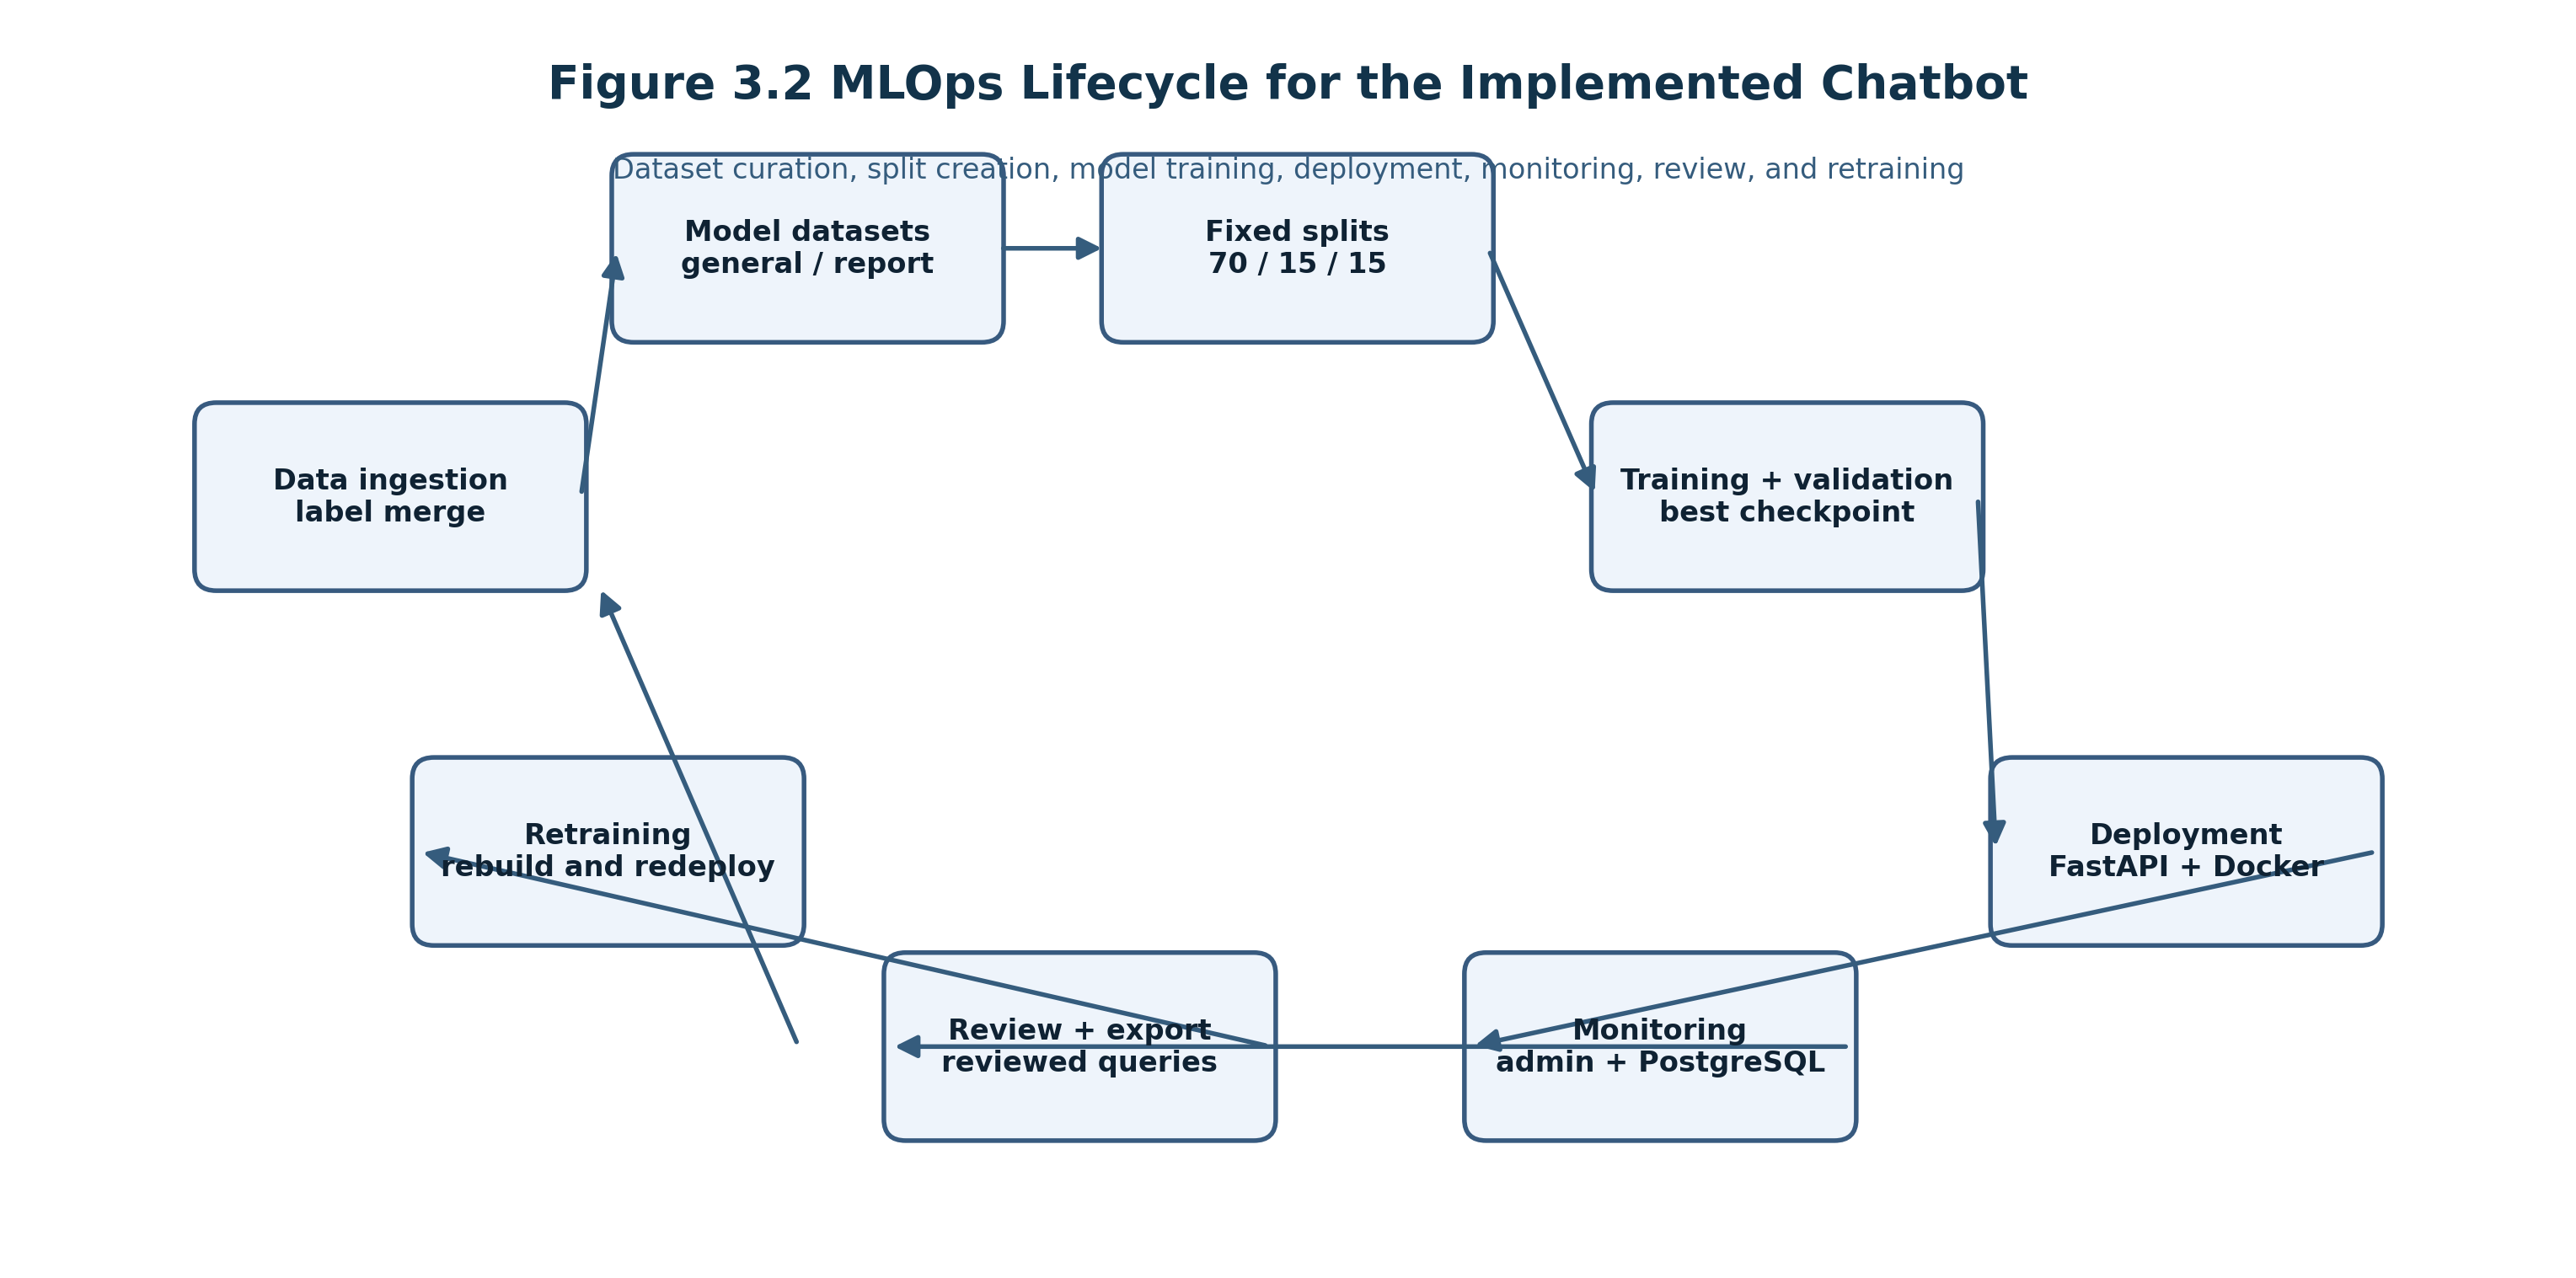
\includegraphics[width=0.88\linewidth]{figures/mlops_lifecycle.png}
    \caption{MLOps lifecycle used in the implemented chatbot project.}
    \label{fig:mlops-lifecycle}
\end{figure}

\begin{figure}[H]
    \centering
    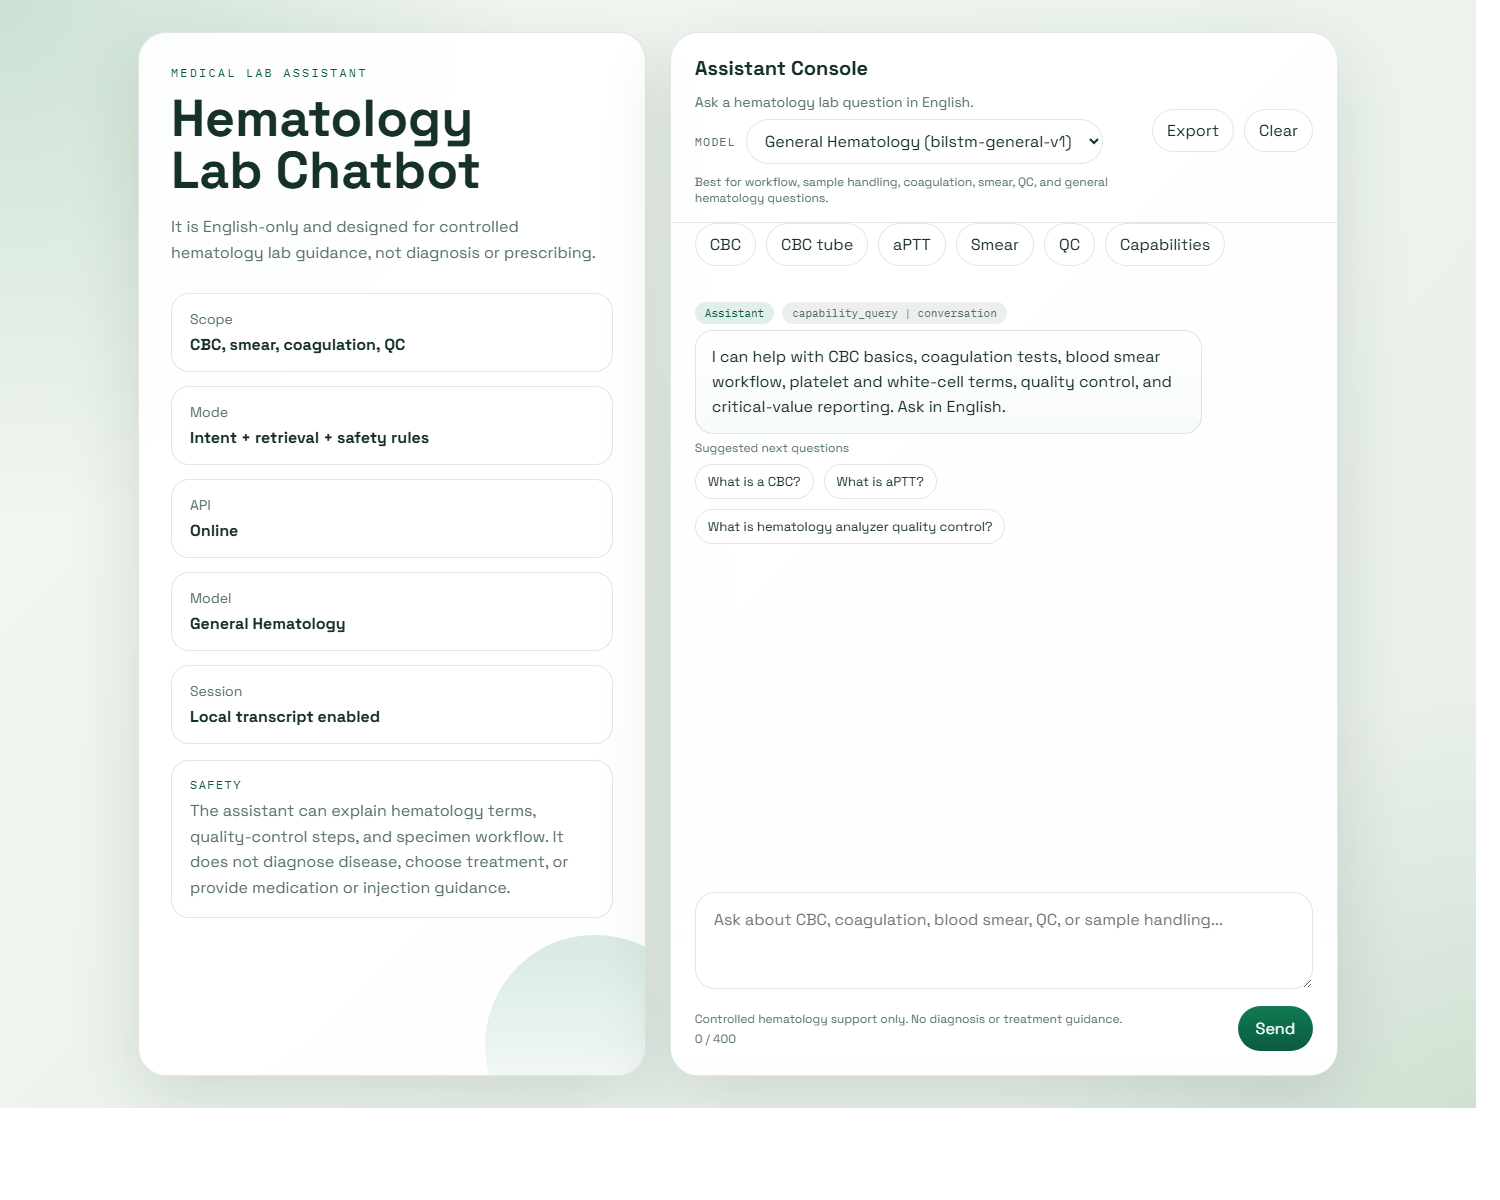
\includegraphics[width=0.74\linewidth]{figures/chat_ui.png}
    \caption{Implemented browser-based chat interface.}
    \label{fig:chat-ui}
\end{figure}

The deployment stack used FastAPI for the HTTP API, PostgreSQL for persistent log storage, static web assets for the chat and admin UIs, and Docker Compose for production-style service composition. The admin console was designed explicitly around MLOps concerns. It included sections for overview metrics, inference trace, data preprocessing, and review queue. Metrics included fallback rate, guardrail rate, low-confidence rate, retrieval rate, and auto-switch rate.

The inference trace view was particularly useful because it exposed the backend path of a single phrase: normalised text, tokens, vocabulary IDs, hard-rule matches, top intent probabilities, entity matches, retrieval candidates, and final routing decision. This feature turned the model from a black box into a partially inspectable system, which was valuable for both debugging and dissertation evidence.

A retraining pipeline was also implemented. Reviewed production phrases could be exported from PostgreSQL into labelled CSV, merged into the master dataset, used to rebuild derived datasets and fixed splits, and then fed back into model training and evaluation. In this way, the project satisfied a core MLOps requirement: feedback from live usage could be converted into future model improvement.
